\chapter{Polynomial Methods for Linear Program Solving}

\section{The Ellipsoid Method}

Discovered by \href{http://en.wikipedia.org/wiki/Leonid\_Khachiyan}{Khachiyan} in 1979 it was the first method to show that Linear Programs can be solved in polynomial time. It is unique because it doesn't look at unnecessary constraints and makes it possible to solve some LPs with an exponential number of constraints in polynomial time. In practice it isn't used though, because it is very slow compared to the simplex method.

We'll only show how to solve feasibility, but it is easy to optimise once you can decide feasibility.

\[\{x|Ax\leq b\} = \emptyset?\]

Since the ellpsoid method works with volumes we'll have to make the assumption that either there is no feasible point at all or the set of feasible points has nonzero volume. More precisely we need that the set of feasible points in the ball with radius $4^{nL}$, centered at the origin, has volume at least $2^{-(n+1)L}$. $L$ is defined as 

\[L=n(1+\log C+\log n)\]

and the entries of $A,b$ are bound from above by $C$. This is basically the amount of bits you need to write down the problem description. These numbers may seem a bit magic, but they are needed to prove the polynomial runtime of the method.

It is possible to transform LPs with just a feasible point such that we get this nonempty volume without making infeasible problems feasible, by wiggling the constraints a bit.

Let $S$ be the set of feasible points inside the $n$-dimensional ball of radius $4^{nL}$ centered at the origin. The ellipsoid method maintains an ellipsoid $E$ that contains $S$. We check if the center of the ellipsoid is contained in the feasible region, if yes we're done, else there has to be some constraint that is violated there. We move the constraint to the center and construct a new ellipsoid that contains the half ellipsoid that is "more feasible". See figure \ref{Fig:ellipsoidMovement}.

The central result will be that the volumes of the ellipsoids decreases exponentially.

\begin{figure}[hbt]
\begin{center}
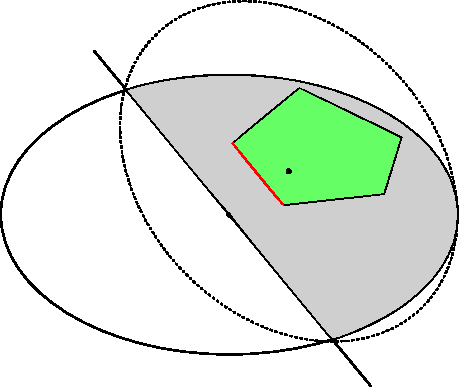
\includegraphics{./images/ellipsoid}
\end{center}
\caption{The final step of the ellipsoid method}
\label{Fig:ellipsoidMovement}
\end{figure}

In pseudocode the algorithm like as follows:

\begin{lstlisting}
E = ball of radius $4^{nL}$ centered at origin
while vol(E) $\geq 2^{-(n+1)L}$
	z = center of E
	if z is feasible return "feasible"
	let $\trans a_ix\leq b_i$ be a violated inequality
	//$\forall x\in S: \trans a_ix\leq b_i \leq \trans a_i z$
	let $1/2E = E\cap \{x|\trans a_i x \leq \trans a_iz\}$
	replace E by the smallest ellipsoid containing $1/2E$
return "infeasible"
\end{lstlisting}

$1/2E$ is the gray area in figure \ref{Fig:ellipsoidMovement}. The problem is how to find the ellipsoid that contains $1/2E$. 

\begin{Def}[Ellipsoid] An ellipsoid with center $z$ is defined as

\[E=\{x|\trans{(x-z)}Q(x-z)\leq 1\}\]

where $Q$ is a positive definite matrix, i.e. $\trans y Q y>0$ except for $y=0$.
\end{Def}

A simpler special case occurs if the initial ellipsoid is the unit ball and the violated constraint is parallel to a coordinate axis. See figure \ref{Fig:ellipsoidStart}

\begin{figure}[hbt]
\begin{center}
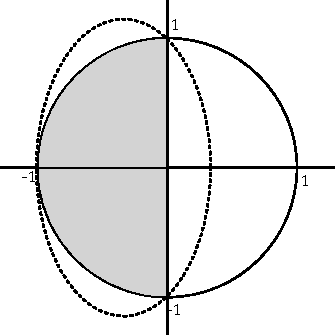
\includegraphics{./images/ellipsoidStart}
\end{center}
\caption{A simpler special case}
\label{Fig:ellipsoidStart}
\end{figure}

\begin{lem} Let $E$ be the unit ball, i.e. $E=\{x|\sum x_i^2\leq 1\}$. Then the smallest ellipsoid that contains $1/2E$, call it $\tilde E$ is

\begin{enumerate}
\item  We want to contain the halfball in an ellipsoid
\[\frac{1}{2}E=E\cap \{x|x_1\leq 0\} \subset \tilde E\]

Where $\tilde E$ can be computed like this
\[\tilde E = \left\{x\left|\left(\frac{n+1}{n}\right)^2\left(x_1+\frac{1}{n+1}\right)^2+\left(\frac{n^2-1}{n^2}\right) \sum_{i=2}^n x_i^2 \leq 1\right.\right\}\]
\item Also the volume of the new ellipsoid decreases.

\[\frac{vol(E')}{vol(E)}\leq f = e^{-1/2n}<1\]
\end{enumerate}
\end{lem}

\begin{pr} The funny terms in the definition of $\tilde E$ come from the case distinction: (1) $x_1=0$ and $\sum_i x_i=1$ (the intersection with the $y$-axis in figure \ref{Fig:ellipsoidStart}) and (2) $x_1=-1$, $x_i=0$. In both cases we want the inequality to be tight. It is easy to verify

\[\left(\frac{n+1}{n}\right)^2\left(0+\frac{1}{n+1}\right)^2+\left(\frac{n^2-1}{n^2}\right) = 1\]

and

\[\left(\frac{n+1}{n}\right)^2\left(-1+\frac{1}{n+1}\right)^2 = 1\]

In the general case the calculation gets more complicated.

Let $x$ be such that $\sum x_i^2\leq 1, -1\leq x_1\leq 0$. We show $x\in E'$
\[\frac{1}{n^2} \left( \underbrace{(n+1)^2}_{n^2+2n+1=n^2-1+2n+2} \left(x_1^2 + \frac{2}{n+1} x_1 + \frac{1}{(n+1)^2}\right) + (n^2-1)\sum_{i=2}^n x_i^2 \right)\]

\begin{align*}
\quad &= \frac{1}{n^2} \left((2n+2)x_1^2 + (2n+2)x_1+1+(n^2-1)\underbrace{\sum_{i=1}^n x_i^2}_{\leq 1} \right)\\
\quad &\leq 1+\frac{1}{n^2}(2n+2)\underbrace{x_1}_{-1\leq x_i\leq 0}(1+\underbrace{x_1}_{\geq -1})\\
\quad &\leq 1
\end{align*}

To prove the part about the volume we first need to recall that the volume of an ellipsiod is proportional to the length if its axes. $E$ has $n$ axes of length $1$, $E'$ has one axis of length $n/n+1$ and $n-1$ axes of length $\sqrt(n^2/n^2-1)$. So it decreases in one dimension, but grows in all the other dimensions. It is nontrivial to show that it shrinks in volume.

%TODO more comments, break in smaller parts
\begin{align*}\frac{vol(E')}{vol(E)}&=\frac{n}{n+1}\cdot \left(\frac{n^2}{n^2-1}\right)^{(n-1)/2}\\
&= \frac{n}{n+1}\cdot \sqrt{\frac{n^2-1}{n^2}} \cdot \left(\frac{n^2}{n^2-1}\right)^{n/2}\\
&=\sqrt{\frac{n^2-1}{(n+1)^2}} \left(\frac{n^2}{n^2-1}\right)^{n/2}\\
&=\sqrt{\frac{(n-1)(n+1)}{(n+1)^2}} \left(\frac{n^2-1+1}{n^2-1}\right)^{n/2}\\
\intertext{It is often helpful to rewrite things as exponentials, because we can bound logarithms more easily:}
&= \sqrt{\frac{n-1}{n+1}} \cdot \exp\left(\frac{n}{2} \ln (1+\frac{1}{n^2-1})\right)\\
\intertext{Now we use the fact that $\ln (1+x)\leq x$ for all $x>0$}
&\leq \sqrt{\frac{n-1}{n+1}} \cdot \exp\left(\frac{n}{2} \cdot \frac{1}{n^2-1}\right)\\
\intertext{We bound $1/(2n-1/n)$ by $1/(2n-1/2)$}
&\leq \sqrt{\frac{n-1}{n+1}} \cdot \exp\left(\frac{1}{2(n-1)}\right)\\
\intertext{Rewrite $n-1$ as $(n+1)-2$}
&=\sqrt{1-\frac{2}{n+1}}\cdot \exp\left(\frac{1}{2(n-1)}\right)\\
\intertext{Write everything as exponentials again to get rid of the squareroot}
&= \exp \left(\ln\left(\sqrt{1-\frac{2}{n+1}}\right)+\frac{1}{2(n-1)}\right)\\
&=\exp \left(\frac{1}{2}\ln \left(1-\frac{2}{n+1}\right) +\frac{1}{2(n+1)}\right)\\
\intertext{Use the trick for the logarithms from above}
&\leq \exp \left(\frac{1}{2} \cdot \frac{-2}{n+1} + \frac{1}{2(n-1)}\right)\\
&= \exp \left(-\frac{1}{n+1}+\frac{1}{2(n-1)}\right)\\
&\approx \exp \left(-\frac{1}{2n}\right)
\end{align*}

So we get

\[f \approx \exp \left(-\frac{1}{2n}\right)\]

\end{pr}

So in the special case for the unit ball we know that the volume decreases as we want.

In the General Case we intersect with a half space $H$ that contains the center $z$ of $E$ in its boundary. We will reduce it to the special case we just proved by

\begin{enumerate}
\item move $z$ to the origin
\[\trans{(x-z)}Q(x-z) \rightsquigarrow \trans xQx\]
\item rotate space such that axes of $E$ align with a coordinate axis. 

For this you need to find the eigenvectors of $Q$, as they are the axes of the ellipsoid. Then you can find their angle with the coordinate axes and use the appropriate \href{http://en.wikipedia.org/wiki/Rotation\_matrix}{rotation matrix}
\item scale the coordinates such that $E$ becomes the unit ball.

Since you already have the eigenvectors at hand from the previous step, calculate their length and scale everything accordingly using a \href{http://en.wikipedia.org/wiki/Scaling\_matrix}{scaling matrix}. This is easy because the axes are parallel to the coordinate axes after the rotation.
\item rotate it again such that $H$ becomes parallel to a coordinate axis
\item compute $E'$
\item reverse back to the original space by doing the transformations backwards.
\end{enumerate}

These steps change the volume of $E$ but they also scale the new ellipsoid $E'$ so that the relative volume of the two doesn't change.

So we proved that the volume of the ellipsoid shrinks by a factor in every step. After $k$ iterations $vol(E)$ is less than $f^k$ times the volume of the initial ball. The initial ball is contained in a cube with side length $2\cdot 4^{nL}$

\[vol(\text{cube}) = (2 \cdot 4^{nL})^n \leq 8^{n^2L}\]

If the $k$th iteration was not the last, i.e. we enter the loop body once more. Then $vol(E)$ must be

\begin{align*}
&2^{-(n+1)L} \leq vol(E) \leq f^k 8^{n^2L} \\
\Leftrightarrow & -(n+1)L  \leq k\log f + 3n^2 L && \log f \approx -\frac{1}{2n}\\
\Leftrightarrow & \frac{k}{2n} \leq (n+1)L+3n^2L \\
\Rightarrow &k = O(n^3L)
\end{align*}

It could be that the real arithmetic we assumed could be exponentially expensive, but since $f$ is fairly far away from $1$ we can round a bit and turn the algorithm to a floating point version without losing correctness.

\begin{Ex}[Travelling Salesman Problem] We're going to formulate the problem as a ILP. For every edge $e$ we have a variable $x_e\in \{0,1\}$. An $x_e$ is $1$ if the corresponding edge is in the tour, $0$ else.

\begin{align*}
\min \quad & \sum_{e\in E} c_e x_e\\
s.t. & \sum_{e\in \delta(v)} x_e = 2 && \forall v\in V\\
	& \sum_{e\in S} \geq 2 && \forall S\subsetneq V, S\neq \emptyset
\end{align*}
\[\delta(v) = \text{set of incident edges to $v$} \qquad \delta(S) = \text{edges with exactly one endpoint in $S$}, S\subseteq V\]

We can relax the problem to $0\leq x_1 \leq 1$ but there still are too many constraints to write the LP down. Using the ellipsoid method however we don't need to have all constraints given at any time. We just have to check whether some constraint is violated and if yes which one. We can check that by solving a mincut problem.
\end{Ex}